\documentclass[12pt]{article}
\usepackage[hmargin=3cm,vmargin=3.5cm]{geometry}

\usepackage[utf8]{inputenc}
\usepackage[french]{babel}
\usepackage[T1]{fontenc}
\usepackage{lmodern}

% Intégration de code Matlab
\usepackage[framed, numbered]{matlab-prettifier}

\usepackage{xcolor}
\usepackage{graphicx}
\usepackage{float}
\usepackage{amsmath}

\usepackage[justification=centering]{caption}

\graphicspath{ {F:/Travail/2A SRI/Estimation} }

\title{Compte rendu de TP\\ \textbf{INTRODUCTION AUX VARIABLES ALEATOIRES}}
\author{Fleytoux Yoann , Aurélien Bernier Levalois}
\date{7 octobre 2016}


% Document
\begin{document}
\maketitle



% Table des matières
\tableofcontents
\vspace{0.6cm}


\section{Présentation du TP}

L'objectif de cette manipulation de Travaux Pratiques est d'illustrer sous MATLAB les notions théoriques vues en cours sur les variables aléatoires.


\section{Variables aléatoires monodimensionnelles}
On se propose de simuler des variables aléatoires Gaussiennes et de visualiser la répartition de leurs échantillons. Pour cela on utilise la fonction randn.
\smallbreak

\textbf{1. }Simuler N =1000 réalisations d'une variable aléatoire Gaussienne scalaire X de moyenne nulle et de variance unité, et placer le résultat dans un vecteur X.Afficher l'histogramme de ces réalisations.
Décrire l'histogramme. Augmenter le nombre de réalisations et commenter.

\smallbreak
\textbf{Réponse:}
\begin{lstlisting}[style=Matlab-editor]
N = 1000;
X = randn([1, N]);
[counts, centers] = hist(X,100);
bar(centers, counts/N/(centers(2)-centers(1)));
%Les valeurs sont comprises entre -4 et 4, plutot centrees vers 0 mais les resultats ne sont pas distribues uniformement

N = 100000;
X = randn([N, 1]);
[counts, centers] = hist(X,100);
figure
bar(centers, counts/N/(centers(2)-centers(1)));
%Avec un plus grand nombre de realisations, les valeurs sont egalement comprises entre -4 et 4 mais convergent plus vers 0, on observe mieux la cloche caracteristique d'une distribution gaussienne
\end{lstlisting}

\begin{flushleft}
Histogramme pour 1000 réalisations
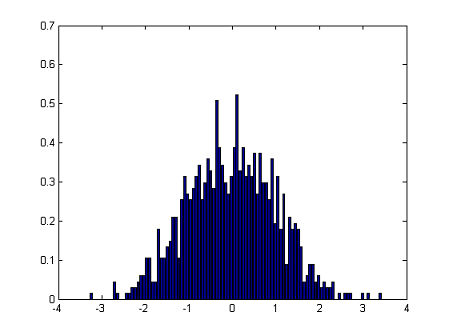
\includegraphics{1_1_1000.PNG}
\end{flushleft}

\begin{flushleft}
Histogramme pour 10000 réalisations
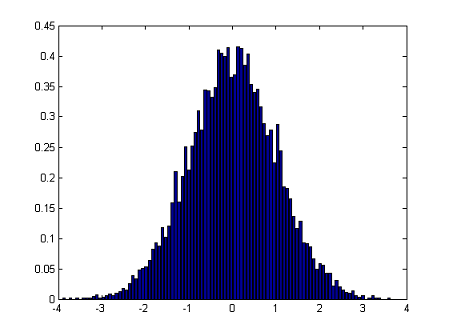
\includegraphics{1_1_10000.PNG}
\end{flushleft}

\textbf{2. }Afin de vérifier l'adéquation de la loi théorique, tracer sur la même figure avec une couleur différente la densité de probabilité théorique, dont la forme est:
\smallbreak
$
p_x(x)=G(x;m_x;\sigma^2)=\dfrac{1}{\sqrt2\pi\sigma} e^{-(x-m_x)^2/(2\sigma^2)}
(1)
$
Choisir des valeurs de x allant de min(x) à max(x) avec un pas de 0.1

\smallbreak
\textbf{Réponse:}
\begin{lstlisting}[style=Matlab-editor]
sigma = 1;%variance (= ecart-type)
meanx = 0;
rangex = (min(X):0.1:max(X));
px = (1/(sqrt(2*pi)*sigma))*exp(-(rangex-meanx).*(rangex-meanx)/(2*sigma*sigma));
hold on
plot(rangex, px, 'r')
hold off
\end{lstlisting}


\begin{flushleft}
Histogramme pour 10000 réalisations avec densité de probabilité théorique
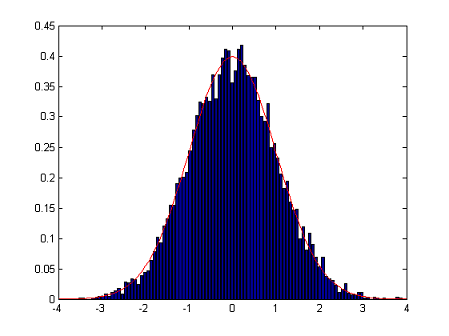
\includegraphics{1_2_10000.PNG}
\end{flushleft}
\smallbreak

Soit la variable aléatoire Gaussienne scalaire Y définie par $Y=10+\sqrt2 X$

\smallbreak

\textbf{3.} Établir la moyenne $m_y$ et la variance $\sigma_y^2$ de Y. En déduire une manière de générer des réalisations de la loi $G(y;m_y,\sigma_y^2)$ au moyen de la commande randn.

\smallbreak
\textbf{Réponse:}
$
E(y)=E(10+\sqrt2 x)=10 + \sqrt 2  m_x
$
Or on sait que $m_x=0$ donc $E(y)=10$
\smallbreak

\begin{math}
var(y)=\sigma ^2 \\
=E[(y-m_y)^2]\\
=E[(10+\sqrt 2 x -m_y)^2]\\
=E[(10+\sqrt 2 x -(10 + \sqrt 2  m_x))^2]\\
=E[(\sqrt 2 x -\sqrt 2  m_x)^2]\\
=E[(\sqrt 2(x -m_x))^2]\\
=E[2(x -m_x)^2]\\
=E[2 \sigma_x]\\
=2
\end{math}

\begin{lstlisting}[style=Matlab-editor]
Y = 10 + sqrt(2)*X;
%mean_Y=mean2(Y)
%variance = var(Y)
mean_Y = 10;
variance = 2;
sigma = sqrt(variance)
gy = mean_Y + sigma*randn([N, 1]);
\end{lstlisting}

\smallbreak

\textbf{4. }Répéter les questions 1 et 2 pour Y. Peut-on retrouver les moments de Y à partir de son histogramme?

\smallbreak
\textbf{Réponse:}
\begin{lstlisting}[style=Matlab-editor]
figure
[counts, centers] = hist(gy,100);
bar(centers, counts/N/(centers(2)-centers(1)));
rangey = (min(Y):0.1:max(Y));
py = (1/(sqrt(2*pi)*sigma))*exp(-(rangey-mean_Y).*(rangey-mean_Y)/(2*sigma*sigma));
hold on
plot(rangey, py, 'r')
\end{lstlisting}


\begin{flushleft}
Histogramme et densité de probabilité théorique pour Y
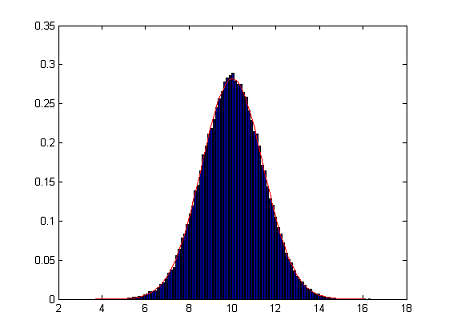
\includegraphics{1_4_10000.PNG}
\end{flushleft}

Non, on ne peut retrouver ces moments à partir de l'histogramme, on ne pourra en donner que des estimations car on n'a un nombre d'expérience fini.
 
\smallbreak

\section{Variables aléatoires bi-dimensionnelles}
On considère des variables aléatoires $X_i =  \begin{pmatrix}
x_i,_1 \\
x_i,_2
\end{pmatrix},i=1,2,...$,à valeurs dans ${\rm I\!R}^2$. Leurs réalisations, générées sous MATLAB, sont stcokées dans des matrices X1,X2,... dont chaque colonne correspond à un tir aléatoire.
\smallbreak
\textbf{5. }Simuler des réalisations de deux variables aléatoires $x_1,_1 , x_1,_2$ indépendantes, Gaussiennes de moyenne nulle et variance unitaire, et les placer dans une matrice X1.

\smallbreak
\textbf{Réponse:}
\begin{lstlisting}[style=Matlab-editor]
N = 100000;
x11 = randn([1, N]);
x12 = randn([1, N]);
X1 = [x11; x12];
%Deux variables aleatoires x11 et x12
\end{lstlisting}
\smallbreak

\textbf{6. }Afficher le nuage des points 2D obtenus. Commenter.

\smallbreak
\textbf{Réponse:}
\begin{lstlisting}[style=Matlab-editor]
plot(X1(1,:),X1(2,:), '.b');
%On voit que le nuage de points est centre sur 0 en abscisses et en ordonnees.
\end{lstlisting}

\clearpage

\begin{flushleft}
Nuage de points de x11 et x12
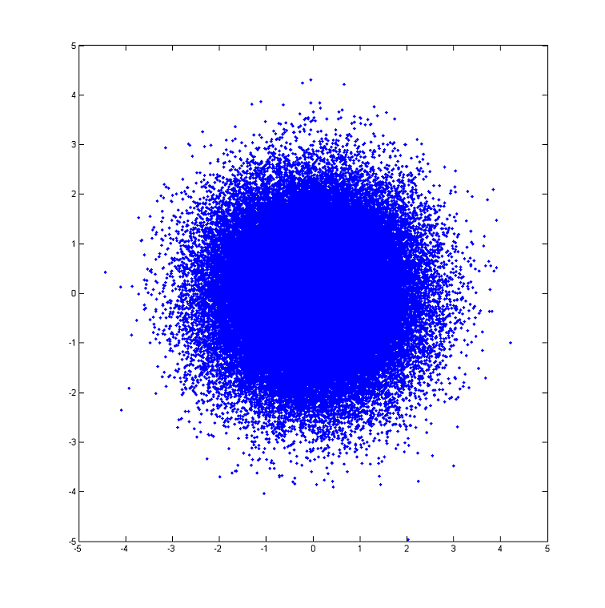
\includegraphics{2_6_100000.PNG}
\end{flushleft}

\smallbreak

\textbf{7. }Répéter la même opération pour deux variables aléatoires$ x_2,_1 , x_2,_2$ indépendantes, où$ x_2,_1$ (resp. $x_2,2$) suit une loi Gaussienne de moyenne 10 et de variance 2 (resp. de moyenne 2 et de variance 0.2) Les réalisations seront placées dans une matrice X2. Commenter.

\smallbreak
\textbf{Réponse:}
\begin{lstlisting}[style=Matlab-editor]
var21 = 2;
var22 = 0.2;
x21 = 10 + sqrt(var21)*randn([1, N]);
x22 = 2 + sqrt(var22)*randn([1, N]);
X2 = [x21; x22];
figure;
plot(X2(1,:),X2(2,:), '.b');
%Ici, le nuage de points est centre sur 10 en abscisses et 2 en ordonnees,
%ce qui est coherent avec les moyennes donnees, on voit egalement que X21 est plus " disperse ", ce qui est coherent avec les variances donnees.
\end{lstlisting}

\begin{flushleft}
 Nuage de points X21 X22
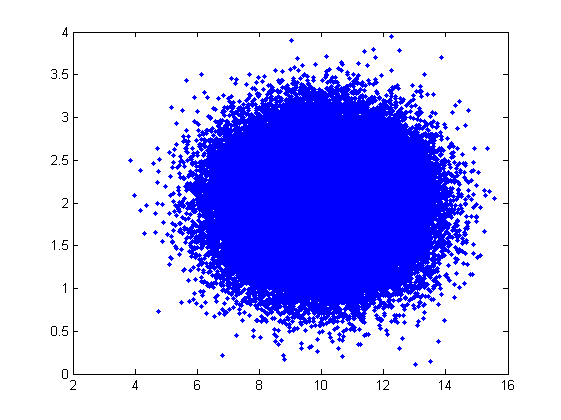
\includegraphics{2_7_10000.PNG}
\end{flushleft}
						


\smallbreak

\textbf{8. }Former la matrice X3 définie par les deux variables aléatoires
$
x_3,_1 = x_1,_1 ; x_3,_2 = x_1,_2 + a x_1,_1;
(2)
$
où $a$ admet successivement les valeurs 1 et 5.

\smallbreak
\textbf{Réponse:}
\begin{lstlisting}[style=Matlab-editor]
x31 = x11;
x321 = x12 + 1*x11;
x325 = x12 + 5*x11;
X31 = [x31; x321];
X35 = [x31; x325];
\end{lstlisting}

\smallbreak

\textbf{9.} Afficher le nuage de points correspondant à X3. Le comparer à celui correspondant à X1. Commenter relativement à l'indépendance des variables aléatoires entrant en jeu.

\smallbreak
\textbf{Réponse:}
\begin{lstlisting}[style=Matlab-editor]
figure;
plot(X31(1,:),X31(2,:), '.b');
figure;
plot(X35(1,:),X35(2,:), '.b');
\end{lstlisting}
Pour X1: variables aléatoires non corrélées et paramètres identiques: on btient un cercle
\smallbreak

\begin{flushleft}
Nuage de points pour X3 avec a = 1
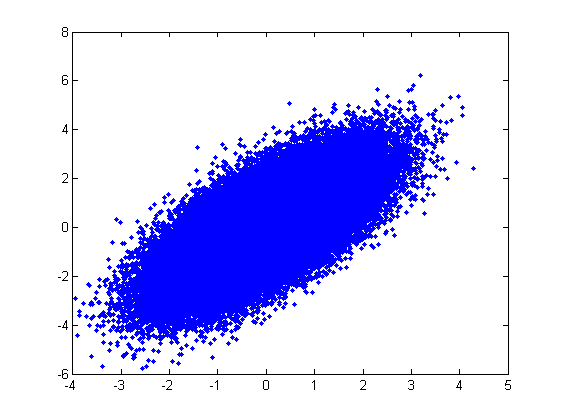
\includegraphics{2_9_A1.PNG}
\clearpage
Nuage de points pour X3 avec a = 5
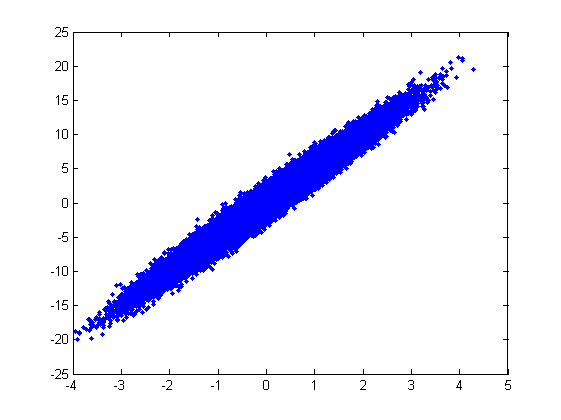
\includegraphics{2_9_A5.PNG}
\end{flushleft}

Pour X31: variables aléatoires corrélées avec un rapport a=1: la corrélation est assez forte (voir l'ellipse de confiance). 
Pour X35: variables aléatoires corrélées avec un rapport a=5: la corrélation est encore plus forte et on observe des ellipses de confiance qui se tassent pour former une droite.

\smallbreak

\textbf{10.} Établir l'expression théorique des moments de
$X_3 =  
\begin{pmatrix}
x_3,_1 \\
x_3,_2
\end{pmatrix}
$
. Les comparer avec leurs estimés empiriques établis par MATLAB au moyen des fonctions mean, cov, etc.

\smallbreak
\textbf{Réponse:}
$
m_3,_1 \\
m_3,_2=m_2,_1 + a m_1,_1
$
\smallbreak

\section{Somme de variables aléatoires}
On considère K variables aléatoires scalaires ${x_k}k-1,...,K$, indépendantes, Gaussiennes centrées de variance unité. K pourra prendre diverses valeurs, e.g, K=3, K=6,etc.
\smallbreak

\textbf{11. }Simuler 10000 réalisations de ces K variables.
Soit la variable aléatoire $y=\sum_{k-1}^{K} x_k$

\smallbreak
\textbf{Réponse:}
\begin{lstlisting}[style=Matlab-editor]
N = 10000;
K3 = 3;
X3 = randn([K3, N]);
Y3 = sum(X3);

\end{lstlisting}


\smallbreak

\textbf{12.} Tracer l'histogramme des réalisations de y (K=3).

\smallbreak
\textbf{Réponse:}
\begin{lstlisting}[style=Matlab-editor]
Y3 = sum(X3);

[counts, centers] = hist(Y3,100);
bar(centers, counts/N/(centers(2)-centers(1)));
\end{lstlisting}
\begin{flushleft}
Histogramme des réalisations de y (K=3)
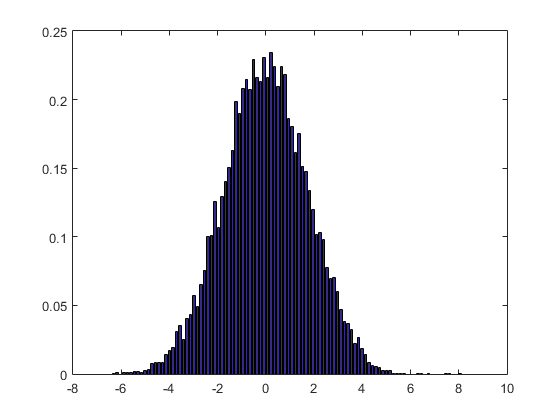
\includegraphics{3_12.PNG}
\end{flushleft}


\smallbreak

\textbf{13.} Quelle loi suit la variable y (type, moyenne, variance)? Superposer la densité de probabilité de y avec son approximation empirique.

\smallbreak
\textbf{Réponse:}

\begin{lstlisting}[style=Matlab-editor]
sigma = sqrt(((1/N)*sum(Y3*Y3')))
meanx3 = 0;
rangey3 = (min(Y3):0.1:max(Y3));
py3 = (1/(sqrt(2*pi)*sigma))*exp(-(rangey3-meanx3).*(rangey3-meanx3)/(2*sigma*sigma));
hold on;
plot(rangey3, py3, 'r')
\end{lstlisting}

\begin{flushleft}
Densité de probabilité de y avec son approximation empirique (k=3)
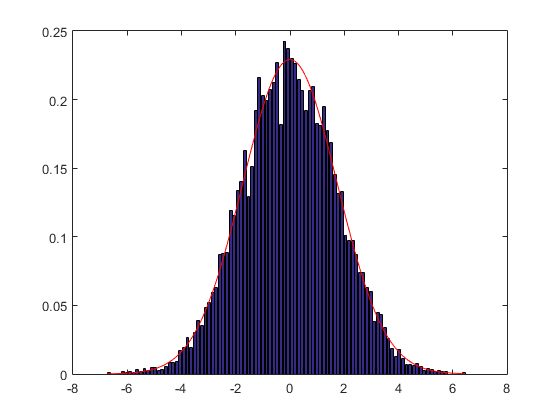
\includegraphics{3_13.PNG}
\end{flushleft}

\begin{flushleft}
Densité de probabilité de y avec son approximation empirique (k=10)
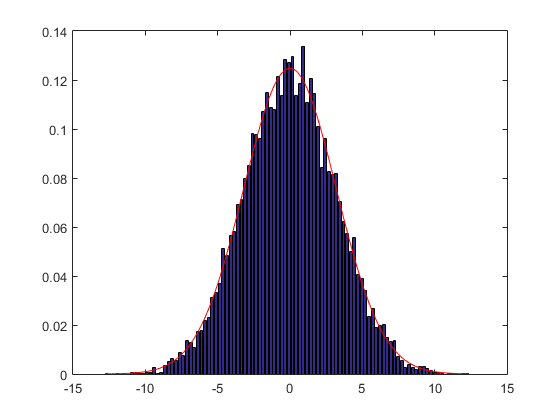
\includegraphics{3_13_10.PNG}
\end{flushleft}

\begin{flushleft}
Densité de probabilité de y avec son approximation empirique (k=50)
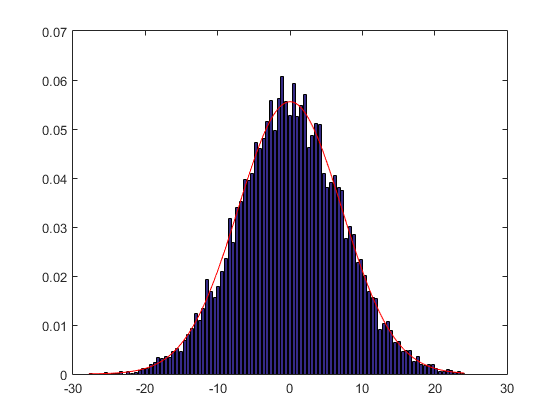
\includegraphics{3_13_50.PNG}
\end{flushleft}

On observe que c'est une loi gaussienne. Sa moyenne sera la somme des moyennes des K variables aléatoires et sa variance, la somme des variances des k variables aléatoires (car les K variables sont indépendantes).
\smallbreak

Soit la variable aléatoire $z = \sum_{k-1}^{K} x_k^2$. La fonction suivante correspond à la densité de probabilité d'une loi $\chi^2$ à K degrés de liberté:
$
p_z(z)=\chi_K^2(z)=\dfrac{z^{(K/2)-1} e^{-z/2}}
{2^{K/2} \Gamma (K/2)}$
où $\Gamma$ désigne la fonction Gamma.
\smallbreak
\textbf{14. }Tracer les histogrammes des réalisations de z pour diverses valeurs de K.

\smallbreak
\textbf{Réponse:}

\begin{lstlisting}[style=Matlab-editor]
X_chi2=X3.*X3;
z=sum(X_chi2);
[counts, centers] = hist(z,100);
bar(centers, counts/N/(centers(2)-centers(1)));
\end{lstlisting}

\clearpage

\begin{flushleft}
Histogrammes des réalisations de z pour K=3
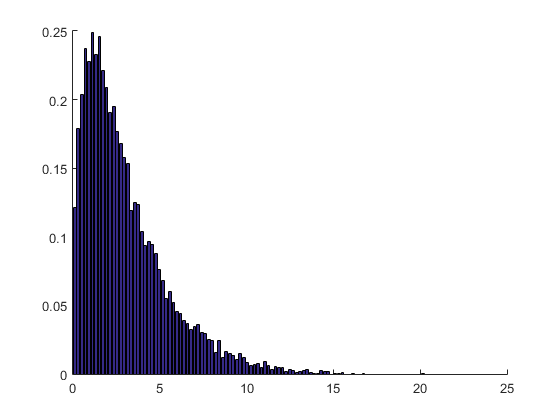
\includegraphics{3_14.PNG}
\end{flushleft}

\smallbreak

\textbf{15. }Superposer la densité de probabilité de z avec son approximation empirique. Commenter.

\smallbreak
\textbf{Réponse:}
\begin{lstlisting}[style=Matlab-editor]
hold on
range_z=(min(z):0.1:max(z));
pz=(range_z.^((K3/2)-1).*exp(-range_z/2))/(2^(K3/2)*gamma(K3/2));
plot(range_z,pz,'r');
\end{lstlisting}

\clearpage

\begin{flushleft}
Superposition de la densité de probabilité de z avec son approximation empirique (K=3)
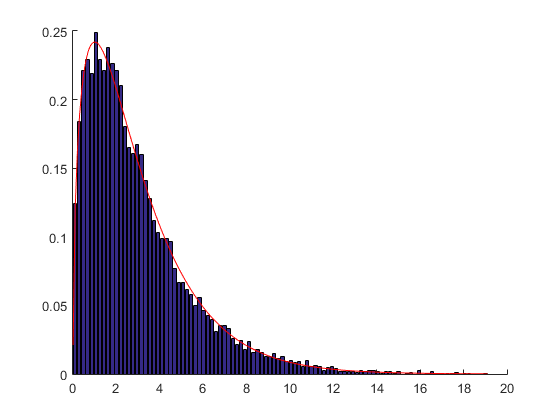
\includegraphics{3_15.PNG}
\end{flushleft}

\clearpage

\begin{flushleft}
Superposition de la densité de probabilité de z avec son approximation empirique (K=10)
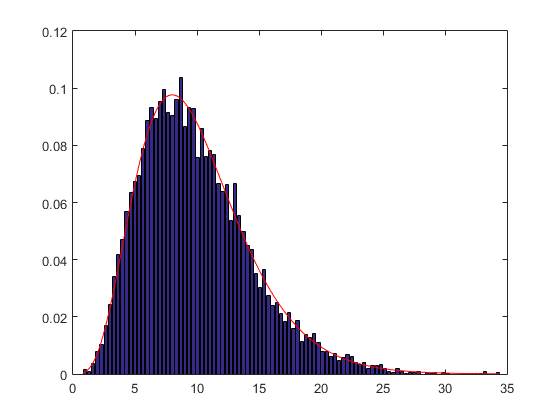
\includegraphics{3_15_10.PNG}
\end{flushleft}

\clearpage

\begin{flushleft}
Superposition de la densité de probabilité de z avec son approximation empirique (K=50)
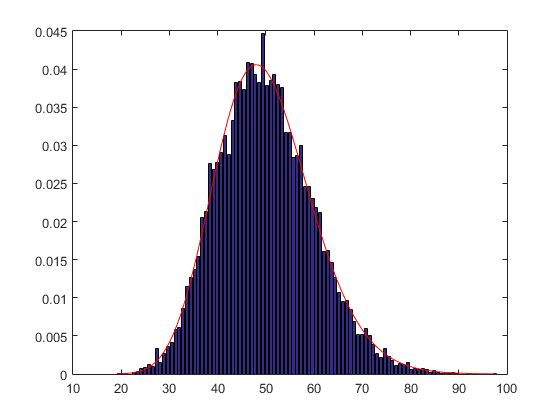
\includegraphics{3_15_50.PNG}
\end{flushleft}

\smallbreak

\textbf{16.} Établir la moyenne et la variance de z en fonction de K.

\smallbreak
\textbf{Réponse:}
$
\\
E(z)=E(\sum_{k=1}^{K}E(X_k^2))=\sum_{k=1}^{K}E[X_k -(m_{xk})^2]=\sum_{k=1}^{K}\sigma_{Xk}=K\\car  \sigma_{Xk}=1\\
$
$
\sigma_z^2=E_z[(z-m_z)^2]=E_z[(\sum_{k=1}^K X_k^2-K)^2]\\
=E_z[(\sum_{k=1}^K (X_k^2) - K)^2]\\
=E_z[((\sum_{k=1}^K (X_k^2))^2 -2 \sum_{k=1}^K (X_k^2) K + K^2]\\
=K^2-2K^2+K^2=0\\ car E(\sum_{k=1}^{K}E(X_k^2))=K
$

\begin{lstlisting}[style=Matlab-editor]
var_z=var(z)
mean_z=mean(z)
\end{lstlisting}

Avec K=3
$
\\ var_z = 6.0247\\
mean_z = 3.0079
$
\smallbreak

\textbf{17.} Renouveler ces calculs pour K = 100. Quel type de loi obtient-on? Quels sont ses moments? Établir un lien avec le théorème central limite.

\smallbreak
\textbf{Réponse:}
\begin{lstlisting}[style=Matlab-editor]
N = 10000;
K = 100;
X = randn([K, N]);
Y = sum(X);
%histo y
[counts, centers] = hist(Y,100);
bar(centers, counts/N/(centers(2)-centers(1)));

sigma = sqrt(((1/N)*sum(Y*Y')))
meanx = 0;
rangey = (min(Y):0.1:max(Y));
py = (1/(sqrt(2*pi)*sigma))*exp(-(rangey-meanx).*(rangey-meanx)/(2*sigma*sigma));
%superposition theorique y
hold on;
plot(rangey, py, 'r')

figure
X_chi2=X.*X;
z=sum(X_chi2);
%histo z
[counts, centers] = hist(z,100);
bar(centers, counts/N/(centers(2)-centers(1)));

hold on
range_z=(min(z):0.1:max(z));
pz=(range_z.^((K/2)-1).*exp(-range_z/2))/(2^(K/2)*gamma(K/2));
%superposition theorique z
plot(range_z,pz,'r');
\end{lstlisting}

\clearpage

\begin{flushleft}
Superposition de la densité de probabilité de y avec
\smallbreak
 son approximation empirique(K=100)
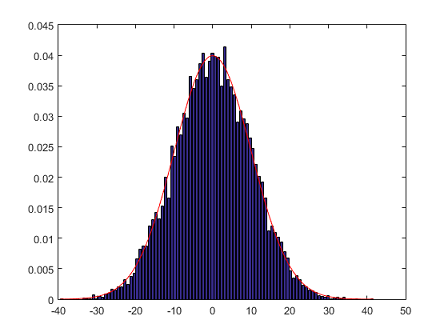
\includegraphics{3_17_y_100.PNG}
\end{flushleft}

\begin{flushleft}
Superposition de la densité de probabilité de z 
\smallbreak
 avec son approximation empirique(K=100)
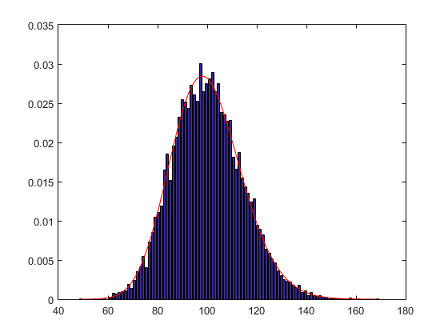
\includegraphics{3_17_z_100.PNG}
\end{flushleft}

\textbf{TODO Quel type de loi obtient-on? Quels sont ses moments? Établir un lien avec le théorème central limite.}

\smallbreak

\end{document}
 